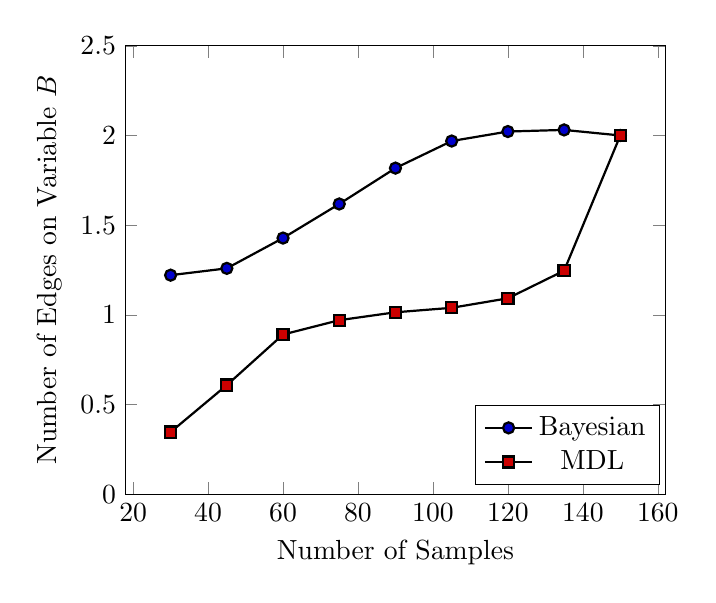
\begin{tikzpicture}
\begin{axis}[
		xlabel = Number of Samples,
		ylabel = Number of Edges on Variable $B$,
		legend style={at={(0.99,0.02)},anchor=south east},
		ymin=0.0, ymax=2.5
]
\addplot+[solid,black,thick] coordinates {
(30, 1.221)
(45, 1.259)
(60, 1.428)
(75, 1.618)
(90, 1.818)
(105, 1.969)
(120, 2.022)
(135, 2.031)
(150, 2.0)
};
\addlegendentry{Bayesian};

\addplot+[solid,black,thick] coordinates {
	(30, 0.346)
	(45, 0.608)
	(60, 0.89)
	(75, 0.97)
	(90, 1.014)
	(105, 1.039)
	(120, 1.092)
	(135, 1.246)
	(150, 2.0)
};
\addlegendentry{MDL};
\end{axis}
\end{tikzpicture}
